\documentclass[a4paper,12pt]{article}
\usepackage[left=2.5cm, right=2.5cm, top=3cm, bottom=3cm]{geometry}
\usepackage[spanish]{babel}
\usepackage{graphicx}

\begin{document}
\title{Presentación}
\author{Johnangel Crespo Leal}
\date{C112}
\maketitle

\section{¿Qué es Moogle! ?}\label{sec:?}
Moogle! es una aplicación *totalmente original* cuyo propósito es buscar inteligentemente un texto en un conjunto de documentos.
Es una aplicación web, desarrollada con tecnología .NET Core 6.0, específicamente usando Blazor como *framework* web para la interfaz gráfica, y en el lenguaje C\#. 

La aplicación está dividida en dos componentes fundamentales:

\begin{itemize}
    \item{`MoogleServer` es un servidor web que renderiza la interfaz gráfica y sirve los resultados .}
    \item{`MoogleEngine` es una biblioteca de clases donde está implementada la lógica del algoritmo de búsqueda (es donde únicamente se trabajó en este proyecto).}
\end{itemize}

\subsection{MoogleEngine}\label{sub:engine}
En este directorio está compuesto por las clases:
\begin{itemize}
    \item{Moogle (editada)}
    \item{SearchItem}
    \item{SearchResult}
    \item{Metodos (nueva)}
    \item{TrabajoSinQuery (nueva)}
    \item{Snippet (nueva)}
\end{itemize}

\textbf{Datos:} 
\begin{itemize}
    \item{La explicación de cada método que contiene cada clase se encuentra en el informe del proyecto.}
    \item{Como solo se trabajó en \underline{MoogleEngine}, todo lo que se hable a partir de ahora se encuentra en dicho directorio.}
\end{itemize}

\section{Resumen de funcionalidad}\label{sec:res}
A continuación se explicará en esencia como trabaja el motor de búsqueda integrado en "Moogle!". (Para una explicación más detallada consultar en informe)

El motor de búsqueda utiliza un "modelo vectorial" para hacer que la búsqueda sea aún más rápida y eficiente, TF-IDF para ser más específicos. El TF-IDF (TermFrequency * InverseDocumentFrequency) es una medida utilizada en el procesamiento del lenguaje natural y la recuperación de información, en la cual se multiplica el TF (Term Frequency) de cada palabra en un documento por su respectivo IDF (Inverse Document Frequency) en el corpus de documentos.

\subsection{TF}
TF se refiere a la importancia de un término en un documento particular.

Esta valor de importancia se calcula con la siguiente fórmula:

\begin{equation}
    \mathrm{TF} = \frac{F}{T}
\end{equation}
Donde:
\begin{itemize}
    \item{TF: es la importancia del termino en el documento}
    \item{F: es la cantidad de veces que aparece la palabra en cuestión dentro del documento}
    \item{T: es la cantidad total de palabras que existen en el documento}
\end{itemize}

Dato: Este cálculo se le aplica a cada palabra de cada documento por separado, por lo que una palabra que se repita en más de un documento puede tener distintos valores de TF relativos a cada documento.

\subsection{IDF}
IDF es una medida que indica la importancia de un término en una colección de documentos. Un término que aparece en muchos documentos tendrá un valor IDF bajo mientras que un término que aparece en pocos documentos tendrá un valor IDF alto.

El valor de IDF de un término se calcula con la siguiente fórmula:

\begin{equation}
    \mathrm{IDF} = \log_{10} (\frac{N}{D})
\end{equation}
Donde:
\begin{itemize}
    \item{IDF: es la importancia de un término en una colección de documentos.}
    \item{N: es el número total de documentos en la colección}
    \item{D: es el número de documentos que contiene el termino en cuestión}
\end{itemize}

Dato: Este cálculo es global, es decir, cada palabra que se encuentre en el corpus de documentos tiene uno y solo un valor de IDF.

\subsection{Cálculo de similitud del coseno}
Una de las claves del Modelo Vectorial es precisamente la posibilidad de determinar el ángulo que forman los vectores de los documentos y de la consulta que se está comparando, véase Figura 1.

\begin{figure}[h]
    \center
    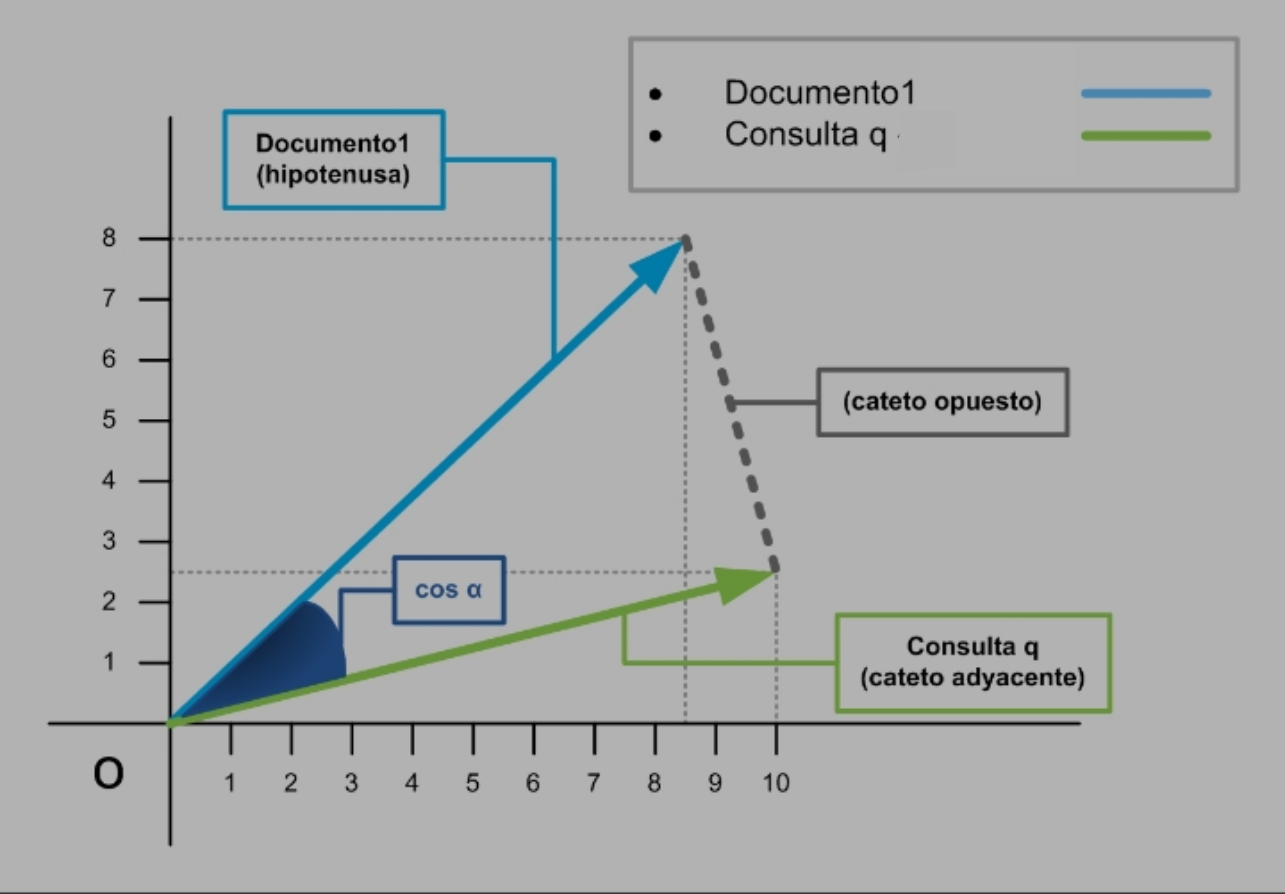
\includegraphics[width=14cm]{grafica.png}
    \caption{El ángulo del coseno}
\end{figure}

Es posible medir cuál es la desviación de un documento con respecto a una consulta por el número de grados del ángulo que forman. Esto es posible porque se crea una estructura triangular a la que se aplica el cálculo del ángulo que forma la hipotenusa (en este caso el vector del documento1) y el adyacente (el vector \textbf{q} de la consulta dada por el usuario) que resulta ser el coseno del triángulo. En el caso de la Figura 1, se comprueba visualmente cierta distancia del vector de la consulta con el vector de documento 1 , cuando ambos vectores se muestran tan próximos como para superponerse, implicará que el ángulo que forman será menor y que su nivel de coincidencia sea superior, de hecho un coseno de 0 grados implicaría una similaridad máxima.

Por lo tanto, la fórmula aplicada para calcular el coheficiente de similaridad del coseno entre un documento y una consulta es aquella que permite poner en relación los vectores de la consulta y el documento. De hecho el coseno de alfa de un triángulo cualquiera siempre es igual al cateto adyacente entre la hipotenusa. Tomando como clave esa idea, la Figura 2 muestra la misma relación pero esta vez con los pesos (TF*IDF) que forman los vectores del documento y la consulta. De hecho el numerador no deja de ser un producto escalar entre los pesos del documento y la consulta; y el denominador la raíz cuadrada del producto de la sumatoria de los pesos del documento y la consulta al cuadrado. Todo esto se diseñó para poder conseguir un resultado final inferior a 1, de tal manera que el coheficiente fuera de fácil manejo y lectura.

\begin{figure}[h]
    \center
    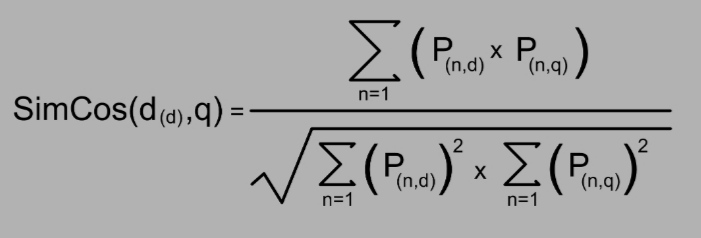
\includegraphics[width=14cm]{formula.jpg}
    \caption{Fórmula para el cálculo de similaridad del coseno}
\end{figure}

\subsection{Snippet}
El snippet es básicamente una porción de texto (en mi caso una oración) que se muestra al usuario debajo de cada documento que posea alguna relevancia con respecto a su búsqueda. Mi forma de hallar el snippet es recorriendo el documento en búsqueda de una oración que contenga el término con mayor TF-IDF de la consulta, en caso de encontrarla se le mostraría al usuario como snippet, caso de no hallar ninguna oración que coincida con dicho término, pasar al segundo término con mayor TD-IDF y repetir el ciclo. (Para más información ver el informe o el código dentro de la clase Snippet)

\subsection{Datos extras}
Básicamente (en esencia) esto es lo que utiliza el motor de búsqueda de Moogle! para realizar la búsqueda de la manera más eficiente y proporcionar un snippet válido. Mi código utiliza todo lo dicho mediante todas las clases mencionadas al principio de la presentación (Todos los detalles importantes se encuentran en el informe así como en los comentarios dentro del código) 
\end{document}
















